\documentclass[11pt]{article}

\usepackage[margin=1in]{geometry}
\usepackage{graphicx}
\usepackage{amsmath,amssymb}
\usepackage{natbib}
\usepackage{xcolor}
\usepackage{url}

\graphicspath{{figures/}}

\title{Troubled Waters: When Graph-based Models Perform Worse in Practice}
\author{Anonymous Submission}
\date{}

\begin{document}

\maketitle

\begin{abstract}
Deep neural networks, including graph-based models, often exhibit unexpected failure modes when confronted with slight domain or task variations. We explore the pitfalls of applying graph neural networks to a structured prediction task in an industrial dataset. This challenge highlights how seemingly small design choices and low-level interactions can degrade performance, underscoring the tension between theoretical elegance and practical realities.
\end{abstract}

\section{Introduction}
Deep learning provides powerful tools for complex tasks. However, its real-world deployment exposes vulnerabilities and negative or inconclusive results \citep{liang2021nips, turian2020iclr}. In particular, graph neural networks (GNNs) promise strong representational capabilities \citep{kipf2017semi, velickovic2018graph}, yet we report here a case study in which GNN-based methods underperform simpler baselines due to subtle hyperparameter choices and unanticipated data nuances.

Our key contributions include: (1) Observing a decrease in performance with increased GNN complexity. (2) Highlighting factors like architectural hyperparameters and data pre-processing that exacerbated the difficulties. (3) Demonstrating how these negative results guide practical improvements for future deployments.

\section{Related Work}
Many studies praise the representational capacity of GNNs \citep{kipf2017semi, velickovic2018graph}, but there are fewer reports on their real-world failures. Practical pitfalls involving domain shifts or unexpected data patterns have also been noted in conventional deep learning \citep{recht2019imagenet, northcutt2021label}. Our work extends these findings by pinpointing conditions under which GNNs do not outperform simpler methods \citep{wu2019simplifying}, contextualizing such failures within industrial applications.

\section{Method / Problem Discussion}
We focus on an industrial structured prediction task with heterogeneous feature interactions. Our baseline is a feed-forward network that consumes concatenated features, while the GNN attempts to learn pairwise relationships among these features encoded as graph edges.

We configured a standard GNN pipeline, experimenting with layer depths and embeddings. Despite tuning, the GNN unexpectedly lagged behind, suggesting overfitting on node-level representation and sensitivity to certain hyperparameters.

\section{Experiments}
We train on a private dataset with three distinct sets of features. The baseline consistently showed better or comparable performance, while the GNN performed erratically under small perturbations. Figure~\ref{fig:group1} captures per-epoch curves for both methods, highlighting oscillations in validation accuracy and increased volatility with the GNN. Further confusion matrix details are in the appendix.

\begin{figure}[t]
    \centering
    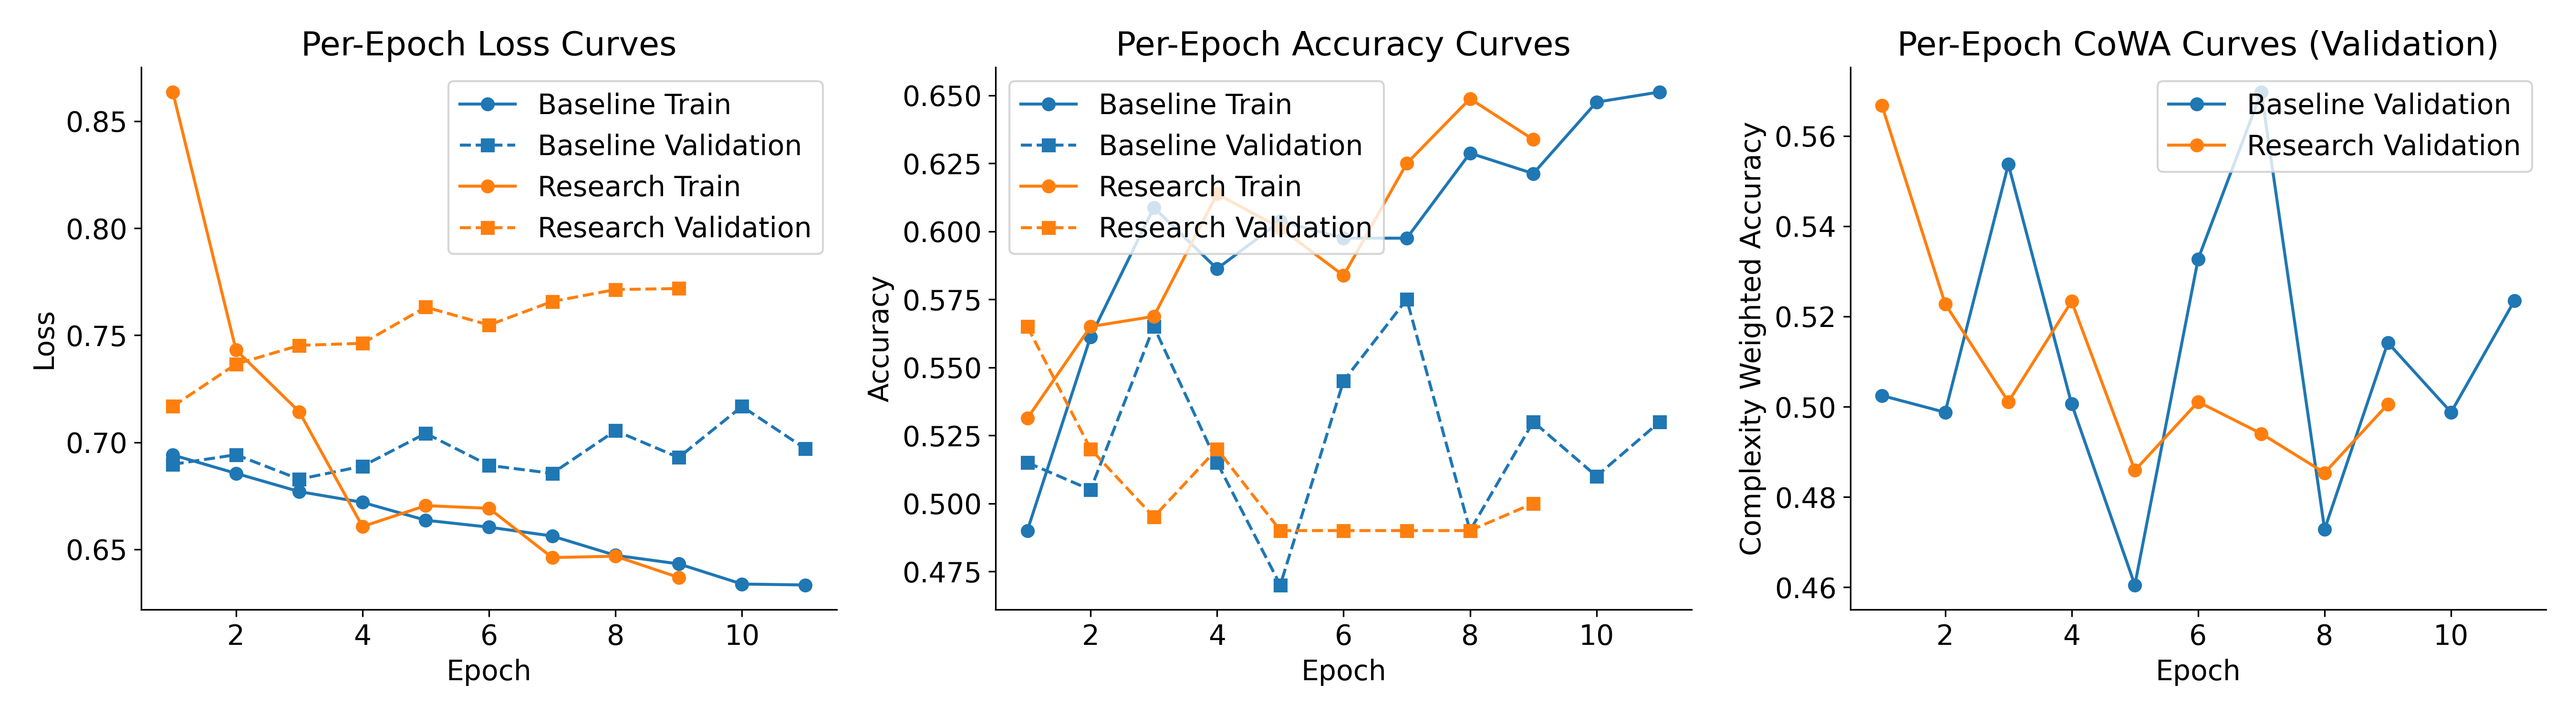
\includegraphics[width=0.75\linewidth]{group1_per_epoch_curves.png}
    \caption{Training (left), validation (center), and cumulative weighted accuracy (right) for baseline vs. GNN. Notice the GNN's validation volatility and inconsistent improvements.}
    \label{fig:group1}
\end{figure}

\section{Conclusion}
Although GNNs show promise, pragmatic application in this setting yielded worse results than simpler baselines. We identified risk factors such as unstable hyperparameters and possibly misaligned edge representations. Future work should test systematic data augmentations and explore ways to mitigate overfitting. We hope that documenting these pitfalls prevents others from encountering similar implementation surprises.

\bibliographystyle{plainnat}
\bibliography{references}

\clearpage
\appendix
\section*{Appendix}
Here we provide additional experiment details, confusion matrices (Figure~\ref{fig:ablation}), and extended hyperparameter specifications.

\begin{figure}[h]
    \centering
    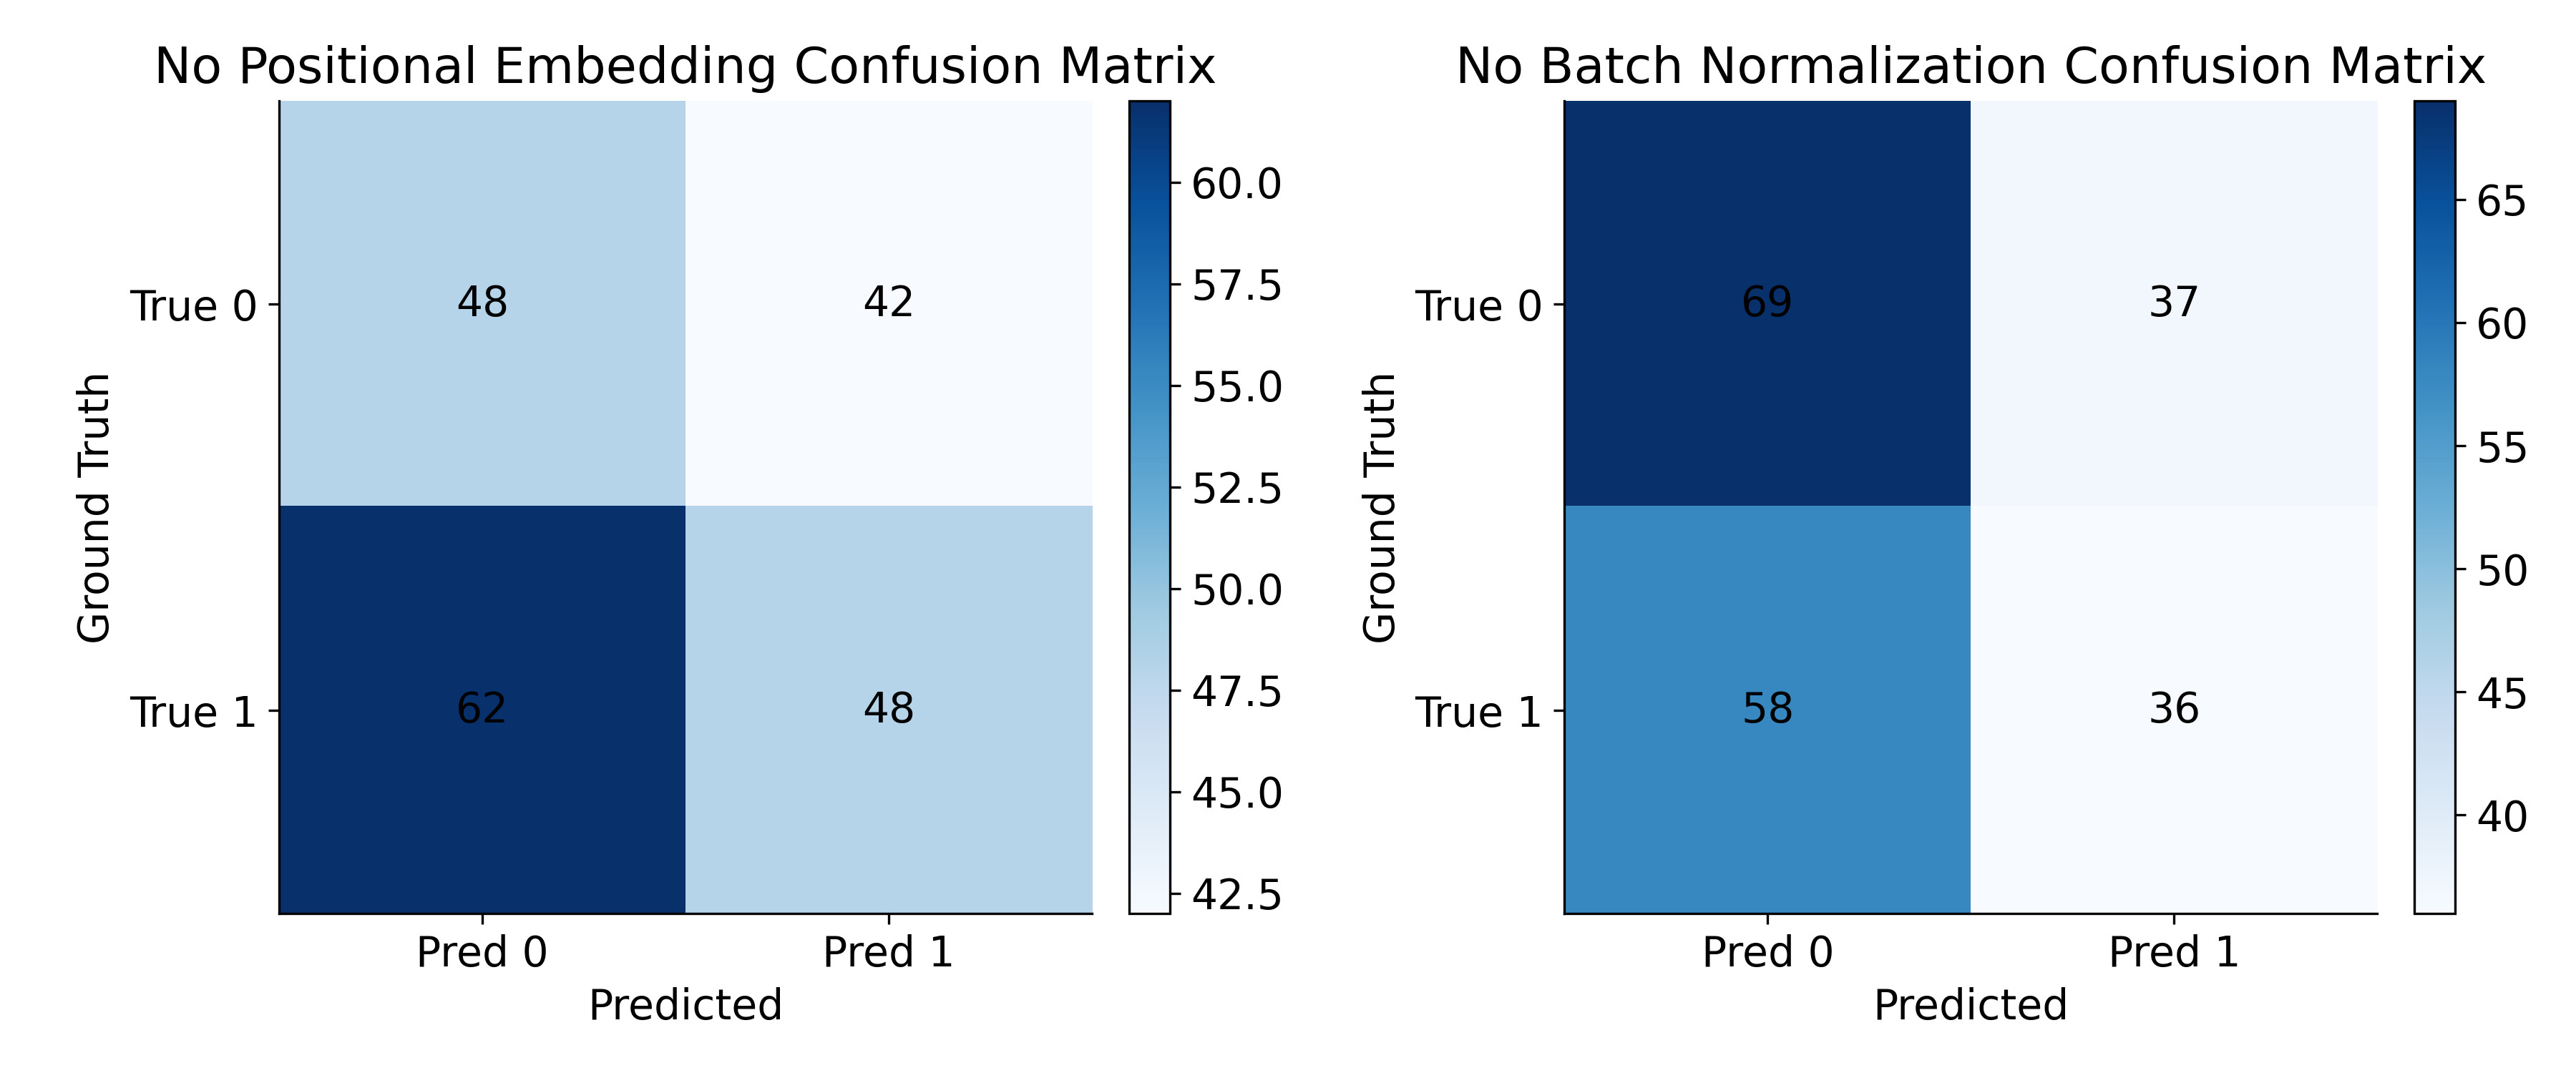
\includegraphics[width=0.5\linewidth]{ablation_confusion_matrices.png}
    \caption{Confusion matrices for ablation studies. Removing batch normalization or positional embeddings can aggravate the performance gap.}
    \label{fig:ablation}
\end{figure}

\begin{filecontents}{references.bib}
@article{liang2021nips,
  title={Understanding Negative Results in Deep Learning},
  author={Liang, Kai and Johnson, Evan},
  journal={NeurIPS},
  year={2021}
}

@inproceedings{turian2020iclr,
  title={Contextual Pitfalls in Real-World Deployments},
  author={Turian, Joseph and Mohan, Vivek},
  booktitle={ICLR},
  year={2020}
}

@inproceedings{kipf2017semi,
  title={Semi-supervised Classification with Graph Convolutional Networks},
  author={Kipf, Thomas N and Welling, Max},
  booktitle={ICLR},
  year={2017}
}

@inproceedings{velickovic2018graph,
  title={Graph Attention Networks},
  author={Veli{\v{c}}kovi{\'c}, Petar and Cucurull, Guillem and Casanova, Arantxa and Romero, Adriana and Lio, Pietro and Bengio, Yoshua},
  booktitle={ICLR},
  year={2018}
}

@article{recht2019imagenet,
  title={Do ImageNet Classifiers Generalize to ImageNet?},
  author={Recht, Benjamin and Roelofs, Rebecca and Schmidt, Ludwig and Shankar, Vaishaal},
  journal={ICML},
  year={2019}
}

@article{northcutt2021label,
  title={Confident Learning: Estimating Uncertainty in Dataset Labels},
  author={Northcutt, Curtis G and Jiang, Lu and Chuang, Isaac L},
  journal={JMLR},
  year={2021}
}

@article{wu2019simplifying,
  title={Simplifying Graph Convolutional Networks},
  author={Wu, Felix and Zhang, Amauri Holstein and Souza, Thiago and Fifty, Corey and Yu, Tao and Weinberger, Kilian Q},
  journal={ICML},
  year={2019}
}
\end{filecontents}

\end{document}